\section{Szeregi liczbowe}

Dany jest ciąg liczbowy $ a_1, a_2, ..., a_n, ... $

Tworzymy jego ciąg sum częściowych :

$$ S_1 = a_1, \ \ S_2 = a_1 + a_2, \ \ S_n = a_1 + a_2 + ... + a_n = \sum\limits_{k = 1}^{n} a_k $$

Jeżeli istnieje granica $ S = \lim_{n \to \infty} S_n $ (skończona lub nieskończona) to oznaczamy ją symbolem 
$ \sum_{k = 1}^{\infty} a_k $. \\

W ogólnym przypadku możemy wziąć ciąg, który zaczyna się od dowolnej liczby całkowitej \linebreak $ n_0 $ : $ a_{n_0}, a_{n_0 + 1}, ..., a_n, ... $
i jego sum częściowych

$$ S_n = a_{n_0}, \ \ S_{n_0 + 1} = a_{n_0} + a_{n_0 + 1}, \ \ S_n = a_{n_0} + a_{n_0 + 1} + ... + a_n = \sum\limits_{k = n_0}^{n} a_k, \ n \geq n_0 $$

$ S = \lim_{n \to \infty} S_n $ jest oznaczana przez $ \sum\limits_{k = n_0}^{\infty} a_k $. \\

\begin{tw}{Definicja} 

Dla ustalonego $ n_0 \in \mathbb{Z} $ obiekt $ \sum\limits_{k = n_0}^{\infty} a_k $ nazywamy \underline{szeregiem liczbowym},
a wartość S (gdy istnieje) jego \underline{sumą}, oznaczaną także przez $ \sum\limits_{k = n_0}^{\infty} a_k $. Mamy wtedy

\[ S_n = a_{n_0}, \ \ S_{n_0 + 1} = a_{n_0} + a_{n_0 + 1}. \ \ S_n = a_{n_0} + a_{n_0 + 1} + ... + a_n + ... = \]
\[ \sum\limits_{k = n_0}^{\infty} a_k = \lim_{n \to \infty} \sum\limits_{k = n_0}^{n} a_k = \lim_{n \to \infty} S_n \]

gdzie

\begin{itemize}
    \item $ S_n $ to $n$ - ta suma szeregu,
    \item $ a_n $ to $n$ - ty wyraz szeregu. \\
\end{itemize}

Terminologia dotycząca sumy $S$ jest taka, jak dla ciągów. Są 3 przypadki : 

\begin{enumerate}
    \item $S$ jest liczbą. Wtedy dany szereg jest \underline{zbieżny} (do $S$).
    \item $S = \infty$ lub $S = -\infty$. Wtedy dany szereg jest \underline{rozbieżny} (do $\infty$ lub $-\infty$).
    \item $ S = \lim_{n \to \infty} S_n $ nie istnieje. Wtedy dany szereg jest \underline{rozbieżny}. \\
\end{enumerate}

\end{tw}

\textbf{Przykłady}

\begin{przyklad}
$$ \frac{1}{2^1} + \frac{1}{2^2} + \frac{1}{2^3} + ... + \frac{1}{2^n} + ... = \suminfty{1} \frac{1}{2^n} 
\textrm { - szereg zbieżny do 1}$$

$$ \frac{1}{2} + \frac{1}{3} + ... + \frac{1}{n} + ... = \sum\limits_{n = 2}^{\infty} \frac{1}{n} 
\textrm { - szereg rozbieżny do } \infty$$

$$ 1 - 1 + 1 - 1 + 1 - 1 + ... = \sum\limits_{n = 0}^{\infty} (-1)^n \textrm{ - szereg rozbieżny} $$
\end{przyklad}

Uwaga. Każdy szereg zaczynający się od indeksu $ n_0 \in \mathbb{Z} $ można przekształcić tak, by zaczynał się od indeksu 1.
Wynika to z równości

$$ \sum\limits_{n = n_0}^{\infty} a_n = \suminfty{1} a_{n + n_0 - 1} $$

$$ \frac{1}{2} + \frac{1}{3} + ... + \frac{1}{n} + ... = \sum\limits_{n = 2}^{\infty} \frac{1}{n} = \sum\limits_{n = 2}^{\infty} a_n
= \suminfty{1} a_{n + 1} = \suminfty{1} \frac{1}{n + 1} $$

\subsection*{Obliczanie sum szeregów}
\addcontentsline{toc}{subsection}{Obliczanie sum szeregów}

Jest to zadanie trudne, a najczęściej niemożliwe, gdyż trudno jest znaleźć bezpośredni wzór na sumy częściowe $S_n$. \\

Niektóre przypadki szczególne.

\begin{enumerate}
    \item Ciąg geometryczny i szereg geometryczny.
    \begin{itemize}
        \item 
        $ a_n = a_1 \cdot q^{n-1} $, gdzie $q$ jest ilorazem ciągu (czyli $a_{n+1} = a_n \cdot q , \ n \geq 1$).
        
        Wtedy

        $$ S_n = a_1 + a_2 + ... + a_n = a_1 \cdot \frac{1 - q^n}{1 - q}, q \neq 1 \ oraz \ S_n = na_1, \ q = 1 $$

        To oznacza, że dla $ a_1 \neq 0 $,

        \item szereg jest zbieżny dla $ -1 < q < 1 $ i jego suma jest $ S = \frac{a_1}{1 - q} $,
        \item szereg jest rozbieżny do $\infty$ lub $-\infty$ dla $ q \geq 1 $, znak zależy od znaku $a_1$,
        \item szereg jest rozbieżny (suma nie istnieje) dla $ q \leq -1 $ \\
    \end{itemize}

    Stąd np.

    $$ \frac{1}{2^1} + \frac{1}{2^2} + \frac{1}{2^3} + ... + \frac{1}{2^n} + ... = \suminfty{1} \frac{1}{2^n} =
    \frac{ \frac{1}{2} }{ 1 - \frac{1}{2} } = 1 \ \textrm{, bo tutaj} \ a_1 = q = \frac{1}{2} $$

    \item Szeregi o wyrazie ogólnym postaci \\
    $ a_n = f(n + 1) - f(n)$ lub $ a_n = f(n) - f(n + 1) $, gdzie $f$ jest pewną funkcją.

    W bardziej ogólnej postaci \\
    \quad $ a_n = f(n + k) - f(n) $ lub $ a_n = f(n) - f(n + k) $, gdzie $ k \in \mathbb{N}^+ $ to tzw. krok. \\
    
    Takie szeregi to tzw. szeregi \underline{teleskopowe} (telescoping series).

    \textbf{Przykłady}

    \begin{przyklad}

    $$ \suminfty{1} \left( \frac{1}{n} - \frac{1}{n + 1} \right) \ \textrm{- tutaj} \ f(x) = \frac{1}{x} $$

    $$ \suminfty{1} \left( \sqrt{n + 1} - \sqrt{n} \right) \ \textrm{- tutaj} \ f(x) = \sqrt{x} $$

    $$ \suminfty{1} \left( \arctan(n) - \arctan(n+2) \right) \ \textrm{- tutaj} \ f(x) = \arctan x $$
    \end{przyklad}

    Dla takich szeregów łatwo wyznacza się wzór na $S_n$. Wyrazy wewnętrzne się upraszczają i zostaje: \\
    suma $k$ pierwszych wartości, \ $f$ suma $k$ ostatnich wartości $f$ (lub na odwrót) \\

\end{enumerate}

\begin{przyklad} D
Dla $ \suminfty{1} \left( f(n) - f(n + 1)) \right) $ mamy

$$ S_n = f(1) - \textcolor{red}{f(2)} + \textcolor{red}{f(2)} - \textcolor{blue}{f(3)} + \textcolor{blue}{f(3)} - 
\textcolor{green}{f(4)} + ... + \textcolor{purple}{f(n)} - f(n + 1) = f(1) - f(n + 1) $$

Jeżeli istnieje granica $ G = \lim_{x \to \infty} f(x) $ to mamy

$$ S = \lim_{n \to \infty} S_n = \lim_{n \to \infty} \left( f(1) - f(n + 1) \right) = f(1) - G $$
\end{przyklad}

\begin{przyklad}

Wyznaczyć sumę $ \suminfty{1} \frac{1}{n^2 + n} $

Wyraz ogólny nie ma postaci różnicy więc trzeba ją stworzyć.

Używając rozkładu na ułamki proste dostajemy

$$ \frac{1}{n^2 + n} = \frac{1}{n(n+1)} = \frac{A}{n} + \frac{B}{n+1} = ... = \frac{1}{n} - \frac{1}{n+1} $$

Zatem 

$$ \suminfty{1} \frac{1}{n^2 + n} = \sum\limits_{n=1}^{\infty} \left( \frac{1}{n} - \frac{1}{n+1} \right) $$

I to daje

$$ S_n = \left( \frac{1}{1} - \frac{1}{2} \right) + \left( \frac{1}{2} - \frac{1}{3} \right) + \left( \frac{1}{3} - \frac{1}{4} \right)
+ ... + \left( \frac{1}{n} - \frac{1}{n+1} \right) = \frac{1}{1} - \frac{1}{n+1}  $$ 

$$ \lim_{n \to \infty} S_n = 1 = \suminfty{1} \frac{1}{n^2 + n} $$
\end{przyklad}

\subsection*{Własności szeregów zbieżnych}
\addcontentsline{toc}{subsection}{Własności szeregów zbieżnych}

\begin{tw}{Twierdzenie}

Jeżeli szeregi $ \sum\limits_{n = n_0}^{\infty} a_n $ oraz $ \sum\limits_{n = n_0}^{\infty} b_n $ są zbieżne to zbieżne są szeregi
$ \sum\limits_{n = n_0}^{\infty} (a_n + b_n) $ \linebreak oraz $ \sum\limits_{n = n_0}^{\infty} (c \cdot a_n), \ c \in \mathbb{R} $. \\

Ponadto

\begin{itemize}
    \item $ \sum\limits_{n = n_0}^{\infty} (a_n \pm b_n) = \sum\limits_{n = n_0}^{\infty} a_n \pm \sum\limits_{n = n_0}^{\infty} b_n $
    \item $ \sum\limits_{n = n_0}^{\infty} (c \cdot a_n) = c \sum\limits_{n = n_0}^{\infty} a_n $ \\
\end{itemize}

Prawdziwe są także analogiczne twierdzenia prowadzące do arytmetyki granic nieskończonych, gdy nie pojawiają się symbole nieoznaczone.
\end{tw}

Na przykład gdy $ \sum\limits_{n = n_0}^{\infty} a_n = \infty $ \ oraz \ $ \sum\limits_{n = n_0}^{\infty} b_n = b \in \mathbb{R} $ \ to 

$$ \sum\limits_{n = n_0}^{\infty} (a_n \pm b_n) = \sum\limits_{n = n_0}^{\infty} a_n \pm \sum\limits_{n = n_0}^{\infty} b_n = \infty $$ \\

Natomiast gdy $ \sum\limits_{n = n_0}^{\infty} a_n = \sum\limits_{n = n_0}^{\infty} b_n = \infty $ to
$ \sum\limits_{n = n_0}^{\infty} (a_n - b_n) $ może być zarówno zbieżny jak i rozbieżny i nie ma sensu równość

$$ \sum\limits_{n = n_0}^{\infty} (a_n - b_n) = \sum\limits_{n = n_0}^{\infty} a_n - \sum\limits_{n = n_0}^{\infty} b_n $$ \\

\begin{tw}{Twierdzenie}

Zmiana wartości $n_0$ nie wpływa na zbieżność/rozbieżność szeregu $ \sum\limits_{n = n_0}^{\infty} a_n $.

Może mieć wpływ na wartość jego sumy.
\end{tw}

Stąd wynika np., że szeregi $ \suminfty{1} a_n $ i $ \sum\limits_{n = 100}^{\infty} a_n $ są albo oba zbieżne
albo oba rozbieżne do $ \infty $ lub $-\infty$ albo oba rozbieżne.

To też oznacza, że na podstawie kilku pierwszych wyrazów ciągu/szeregu

\textbf{NIC NIE MOŻNA POWIEDZIEĆ} o jego zbieżności \\

\begin{blad}{Popularny błąd}

"Liczymy wartości $ a_1, a_2, a_3, a_4, a_5$ . Wychodzi ciąg malejący i dodatni.

\textcolor{red}{Zatem szereg jest zbieżny}". \textbf{GAME OVER...} 
\end{blad}

\begin{tw}{Twierdzenie}

Dla ustalonego $ n_0 \in \mathbb{N}^+ $ i $ p \in \mathbb{R} $ szereg $ \sum\limits_{n = n_0}^{\infty} \frac{1}{n^p} $
jest zbieżny dla $ p > 1 $ i rozbieżny do $\infty$ dla $p \leq 1$.  \\

W przypadku kiedy sumy szeregu nie da się wyznaczyć w sposób dokładny można to zrobić w sposób przybliżony, pod warunkiem, że wiemy,
że szereg jest zbiezny. \\

Kryteria zbieżności to twierdzenia opisujące warunki dostateczne zbieżności lub rozbieżności danej klasy szeregów. Najczęściej mają postać
implikacji ale \textbf{NIE} równoważności. \\

Oznacza to zwykle własności postaci

\quad warunek zachodzi $ \Rightarrow $ szereg jest zbieżny/rozbieżny,

\quad warunek nie zachodzi $\Rightarrow$ nic nie wiemy o zbieżności/rozbieżności szeregu
\end{tw}

\subsection*{Popularne kryteria zbieżności szeregów}
\addcontentsline{toc}{subsection}{Popularne kryteria zbieżności szeregów}

0. Warunek konieczny zbieżności szeregów \\ 

\begin{tw}{Twierdzenie}

Jeżeli szereg $ \sum\limits_{n = n_0}^{\infty} a_n $ jest zbieżny to $ \lim_{n \to \infty} a_n = 0 $.
\end{tw}

Dowód 

Dla $ n \geq n_0 + 1 $ mamy $ S_n = a_{n_0} + a_{n_0 + 1} + ... + a_{n - 1} + a_n $ oraz 
$ S_{n - 1} = a_{n_0} + a_{n_0 + 1} + ... + a_{n - 1} $,

Stąd

$$ S_n - S_{n - 1} = a_n $$ \\

Jeżeli szereg $ \sum\limits_{n = n_0}^{\infty} a_n $ jest zbieżny to $ \lim_{n \to \infty} S_n = \lim_{n \to \infty} S_{n - 1} = S \in \mathbb{R} $.
To daje

$$ \lim_{n \to \infty} a_n = \lim_{n \to \infty} (S_n - S_{n - 1}) = \lim_{n \to \infty} S_n - \lim_{n \to \infty} S_{n - 1} = S - S = 0 $$ \\

Transpozycja tego twierdzenia daje warunek równoważny do zastosowania praktycznego :

Jeżeli $ \lim_{n \to \infty} a_n \neq 0 $ to szereg $ \sum\limits_{n = n_0}^{\infty} a_n $ nie jest zbieżny przy czym

\begin{itemize}
    \item gdy $ \lim_{n \to \infty} a_n > 0 $ to $ \sum\limits_{n = n_0}^{\infty} a_n = \infty $
    \item gdy $ \lim_{n \to \infty} a_n < 0 $ to $ \sum\limits_{n = n_0}^{\infty} a_n = -\infty $ 
\end{itemize}

\textbf{Uwaga. To jest tylko implikacja!}

Jeżeli $ \lim_{n \to \infty} a_n = 0 $ to jeszcze \textbf{NIC NIE WIEMY} o szeregu.

Na przykład szeregi $ \sum\limits_{n = n_0}^{\infty} \frac{1}{n^p} $ mają $ \lim_{n \to \infty} \frac{1}{n^p} = 0 $
dla wszystkich $ p > 0 $ ale niektóre z tych szeregów są zbieżne, a niektóre rozbieżne. \\

\begin{blad}{Popularny błąd}

"$\lim_{n \to \infty} a_n = 0 $ \textcolor{red}{zatem szereg jest zbieżny}". \textbf{GAME OVER...}
\end{blad}

Szeregi o wyrazach nieujemnych

$$ \sum\limits_{n = n_0}^{\infty} a_n, \ a_n \geq 0 $$

Wtedy $ S_n = a_{n_0} + a_{n_0 + 1} + ... + a_{n - 1} + a_n $ jest ciągiem niemalejącym zatem suma szeregu
$ \sum\limits_{n = n_0}^{\infty} a_n = \lim_{n \to \infty} S_n $ zawsze istnieje. Może być to liczba lub $\infty$.

Podobnie dla szeregów o wyrazach niedodatnich $ \sum\limits_{n = n_0}^{\infty} a_n, \ a_n \leq 0 $, suma zawsze istnieje
i rozbieżność oznacza rozbieżność do $-\infty$. \\

\begin{przyklad}
Następujące szeregi nie są zbieżne

$$ \suminfty{1} 1, \ \ \suminfty{1} (n^2 + 2n), \ \
\suminfty{1} \frac{n+1}{n+2}, \ \ \suminfty{1} \left(1 + \frac{1}{n} \right)^n , \ \ 
\suminfty{1} (-1)^n , \ \ \suminfty{1} \sin n$$
\end{przyklad}

Dla szeregów o wyrazach nieujemnych mamy dwa kolejne kryteria zbieżności.

\begin{enumerate}
    \item Kryterium porównawcze
    \item Kryterium ilorazowe \\
\end{enumerate} 

\subsection*{Twierdzenie (kryterium porównawcze)}
\addcontentsline{toc}{subsection}{Twierdzenie (kryterium porównawcze)}

Dane są dwa szeregi $ \sum\limits_{n = n_0}^{\infty} a_n $ oraz $ \sum\limits_{n = n_0}^{\infty} b_n $. Wtedy zachodzą nastepujące
własności.

\begin{enumerate}
    \item (Przypadek zbieżności) Gdy $ \forall n \geq k \geq n_0 \quad 0 \leq a_n \leq b_n $ i $ \sum\limits_{n = n_0}^{\infty} b_n $
    jest zbieżny to $ \sum\limits_{n = n_0}^{\infty} a_n $ też jest zbieżny. Ponadto
    $ 0 \leq \sum\limits_{n = n_0}^{\infty} a_n \leq \sum\limits_{n = n_0}^{\infty} b_n $
    
    \item (Przypadek rozbieżności) Gdy $ \forall n \geq k \geq n_0 \quad 0 \leq b_n \leq a_n $ i $ \sum\limits_{n = n_0}^{\infty} b_n $
    jest rozbieżny to $ \sum\limits_{n = n_0}^{\infty} a_n $ też jest rozbieżny. Ponadto
    $ \sum\limits_{n = n_0}^{\infty} a_n = \sum\limits_{n = n_0}^{\infty} b_n = \infty $

    \item (Przypadek wątpliwy). Gdy $ \forall n \geq k \geq n_0 \quad 0 \leq a_n \leq b_n $ ale $ \sum\limits_{n = n_0}^{\infty} b_n $ jest
    rozbieżny to \textbf{NIC NIE WIEMY} o zbieżności $ \sum\limits_{n = n_0}^{\infty} a_n $

    \item (Przypadek wątpliwy). Gdy $ \forall n \geq k \geq n_0 \quad 0 \leq b_n \leq a_n $ ale $ \sum\limits_{n = n_0}^{\infty} b_n $ jest
    zbieżny to \textbf{NIC NIE WIEMY} o zbieżności $ \sum\limits_{n = n_0}^{\infty} a_n $ \\
\end{enumerate}

Uwagi

\begin{itemize}
    \item $ \sum\limits_{n = n_0}^{\infty} a_n $ jest szeregiem z zadania, $ \sum\limits_{n = n_0}^{\infty} b_n $ tworzymy sami
    \item Porównujemy najczęściej z szeregiem geometrycznym $ \sum\limits_{n = n_0}^{\infty} q^n $ lub z szeregami
    $ \sum\limits_{n = n_0}^{\infty} \frac{1}{n^p} $. Wtedy $a_n$ często ma postać ułamków i możemy spróbować wziąć $b_n$ jako

    \quad \textbf{C $\cdot$ iloraz najwyższych potęg z licznika i mianownika $a_n$} 

    \item Trzeba uważać aby nierówność między $a_n$ i $b_n$ była prawdziwa i nie zapomnieć o dolnym ograniczeniu (0). Ma być
    tak jak w \underline{twierdzeniu o trzech ciągach}

    \item Kryterium nie zawsze jest wygodne w użyciu i trzeba uważać, by nie dostać przypadku wątpliwego, bo wtedy \textbf{trzeba zaczynać od nowa}
    
    \item Warto sprawdzić opisany wyżej iloraz najwyższych potęg i na tej podstawie przewidzieć czy chcemy udowodnić zbieżność
    czy rozbieżność. To pomaga skonstruować odpowiednią nierówność między $a_n$ i $b_n$.
\end{itemize}
\bigskip

\begin{blad}{Popularny błąd -- odpowiedź na podstawie przypadku wątpliwego } 

Na przykład dla szeregu $ \suminfty{1} \frac{1}{n + \sqrt{n}} : $

"Mamy $ 0 \leq \frac{1}{n + \sqrt{n}} \leq \frac{1}{n} $ i szereg $ \suminfty{1} \frac{1}{n} $
jest rozbieżny \textcolor{red}{zatem szereg $\suminfty{1} \frac{1}{n + \sqrt{n}}$ jest rozbieżny}". \\

\textbf{GAME OVER...} To jest przypadek nr 3 (wątpliwy)
\end{blad}

\begin{przyklad}

$$ \sum\limits_{n = 4}^{\infty} \frac{2n - 3}{n^3 - 1} $$

Przewidywanie zbieżności/rozbieżności:

Iloraz najwyższych potęg licznika i mianownika to $ \frac{n}{n^3} = \frac{1}{n^2} $, a szereg $ \sum\limits_{n = 4}^{\infty} \frac{1}{n^2} $
jest zbieżny, bo $ 2 > 1 $. Zatem chcemy udowodnić zbieżność (przypadek 1).

Potrzebujemy więc $ \sum\limits_{n = 4}^{\infty} b_n $ i nierówności $ 0 \leq \frac{2n - 3}{n^3 - 1} \leq b_n $.

Chcemy zwiększyć wyrażenie $ \frac{2n - 3}{n^3 - 1} $ ale tak, by \textbf{zostały najwyższe potęgi}.

Można zwiększyć \underline{licznik} oraz \underline{zmniejszyć mianownik}.

Zwiększamy licznik poprzez wyrzucenie 3.

Zmniejszamy mianownik poprzez zastąpienie 1 czymś większym : wyrażeniem z najwyższą potęgą. Nie można jednak wziąć całego $n^3$
, bo będzie 0 w mianowniku.

Wygrywa wzięcie $ C \cdot n^3 $ np. $ \frac{1}{2} n^3 $, bo dla $ n \geq 4 $ mamy $ \frac{1}{2} n^3 \geq 1 $.

To wszystko daje dla $ n \geq 4 $

$$ 0 \leq \frac{2n - 3}{n^3 - 1} \leq \frac{2n}{n^3 - \frac{1}{2} n^3} $$

Czyli

$$ b_n = \frac{2n}{n^3 - \frac{1}{2}n^3} = 4 \cdot \frac{1}{n^2} $$

\textbf{DZIURA W SKRYPCIE}
\end{przyklad}

\subsection*{Twierdzenie (kryterium ilorazowe)}
\addcontentsline{toc}{subsection}{Twierdzenie (kryterium ilorazowe)}

Dane są dwa szeregi $ \sum\limits_{n = n_0}^{\infty} a_n $ oraz $ \sum\limits_{n = n_0}^{\infty} b_n $.
Ponadto $ \forall n \geq n_0 \ a_n, b_n > 0 $.

Jeżeli istnieje granica $ \lim_{n \to \infty} \frac{a_n}{b_n} $ i jest \textbf{liczbą dodatnią} to wtedy oba
szeregi są zbieżne albo oba rozbieżne do $\infty$. \\

Uwagi

\begin{itemize}
    \item Ciąg $b_n$ tworzymy podobnie jak dla kryterium porównawczego.
    \item Nie ma problemu z nierównościami :) ale za to trzeba umieć liczyć granice.
    \item Granica nie może być ani 0 ani $\infty$: \ $ \lim_{n \to \infty} \frac{a_n}{b_n} = L \in (0, \infty) $.
    
    \textbf{Nie wystarczy warunek $L > 0$ bo $\infty$ także jest $ > 0$.}
    \item Rozwiązanie \textbf{musi zawierać wniosek} "granica ilorazu jest liczbą dodatnią więc oba
    \textbf{szeregi} są zbieżne lub oba rozbieżne" - bez tego będzie niepełne
    
    \item Kryterium zwykle jest wygodniejsze niż porównawcze ale są przykłady, które pójdą z porównawczego ale nie z
    ilorazowego, bo granica ilorazu nie istnieje
    
    Np. \ $ \suminfty{1} \frac{2 + \sin n}{n} $.
\end{itemize}

\begin{przyklad}

Poprzedni przykład raz jeszcze 

$$ \sum\limits_{n = 4}^{\infty} \frac{2n - 3}{n^3 - 1} $$

Bierzemy $ b_n = \frac{n}{n^3} = \frac{1}{n^2} $

$$ \dfrac{a_n}{b_n} = \dfrac{\dfrac{2n - 3}{n^3 - 1}}{\dfrac{1}{n^2}} = \dfrac{2n^3 - 3n^2}{n^3 - 1}
= \dfrac{2 - \dfrac{3}{n}}{1 - \dfrac{1}{n^3}} $$ \\

Stąd $ \lim_{n \to \infty} \frac{a_n}{b_n} = 2 $ - liczba dodatnia.

Zatem oba szeregi są zbieżne lub oba są rozbieżne.

Dalej już analiza $ \sum\limits_{n = 4}^{\infty} \frac{1}{n^2} $ i wniosek jak w kryterium porównawczym :

$ \sum\limits_{n = 4}^{\infty} b_n = \sum\limits_{n = 4}^{\infty} \frac{1}{n^2} $ jest zbieżny bo $ 2 > 1 $.
Zatem $ \sum\limits_{n = 4}^{\infty} \frac{2n - 3}{n^3 - 1} $ też jest zbieżny.
\end{przyklad}

Przykłady o postaci funkcji złożonej $ \sum\limits_{n = n_0}^{\infty} f(b_n) $,

gdzie $ \lim_{n \to \infty} b_n = 0^+ $ oraz $ \lim_{x \to 0^+} f(x) = 0^+ $.

Nowym szeregiem jest szereg z funkcji wewnętrznej $ \sum\limits_{n = n_0}^{\infty} b_n $.

Liczymy granicę 

$$ \lim_{n \to \infty} \frac{f(b_n)}{b_n} = \lim_{x=b \to 0^+} \frac{f(x)}{x} \left[ \frac{0}{0} \right] $$

przy użyciu granic podstawowych lub reguły de l'Hospitala. \\

\begin{przyklad}

$$ \suminfty{1} \left( \sqrt[n]{2} - 1 \right) $$

Mamy $$ \suminfty{1} \left( \sqrt[n]{2} - 1 \right) = \suminfty{1} \left( 2^{\frac{1}{n}} - 1 \right) $$

Więc bierzemy $ b_n = \frac{1}{n} > 0 $.

Liczymy granicę

$$ \lim_{n \to \infty} \frac{2^{\frac{1}{n}} - 1}{\frac{1}{n}} = \lim_{x = \frac{1}{n} \to 0^+} \frac{2^x - 1}{x} = \ln 2 $$ \\

Jest to liczba dodatnia więc oba szeregi są zbieżne lub oba są rozbieżne.

$ \suminfty{1} \frac{1}{n} = \infty $ więc $ \suminfty{1} \left( \sqrt[n]{2} - 1 \right) = \infty $.
\end{przyklad}

3. Kryterium Cauchy'ego.

4. Kryterium d'Alemberta \\

Działają dla szeregów o dowolnych wyrazach. Teza obu kryteriów jest taka sama ale liczymy granice innych wyrażeń.


\subsection*{Twierdzenie (kryterium Cauchy'ego)}
\addcontentsline{toc}{subsection}{Twierdzenie (kryterium Cauchy'ego)}

Dany jest szereg $ \sum\limits_{n = n_0}^{\infty} a_n $ taki, że istnieje granica $ q = \lim_{n \to \infty} \sqrt[n]{|a_n|} $. Wtedy

\begin{enumerate}
    \item Gdy $ 0 \leq q < 1 $ to szereg jest zbieżny.
    \item Gdy $ q > 1 $ to szereg jest rozbieżny
    \item \textbf{(Przypadek wątpliwy)}. Gdy q = 1 to \textbf{NIC NIE WIEMY} o zbieżności szeregu. \\
\end{enumerate}

\textbf{Uwagi}

\begin{itemize}
    \item Do wyznaczenia $q$ przydają się następujące właśności granic
    
    a) Gdy $ \lim_{n \to \infty} a_n $ jest \textbf{liczbą dodatnią} to $ \lim_{n \to \infty} \sqrt[n]{a_n} = 1 $.

    b) $ \forall p \in \mathbb{R} \ \lim_{n \to \infty} \sqrt[n]{n^p} = 1 $.

    \item \textbf{$q$ nie może być ujemne}. $q$ ujemne zwykle oznacza brak modułu na $a_n$.
\end{itemize}


\subsection*{Twierdzenie (kryterium d'Alemberta)}
\addcontentsline{toc}{subsection}{Twierdzenie (kryterium d'Alemberta)}

Dany jest szereg $ \sum\limits_{n = n_0}^{\infty} a_n, \ a_n \neq 0 $, taki, że istnieje granica
$ q = \lim_{n \to \infty} \left| \frac{a_{n + 1}}{a_n} \right| $. Wtedy

\begin{enumerate}
    \item Gdy $ 0 \leq q < 1 $ to szereg jest zbieżny.
    \item Gdy $ q > 1 $ to szereg jest rozbieżny
    \item \textbf{(Przypadek wątpliwy)}. Gdy q = 1 to \textbf{NIC NIE WIEMY} o zbieżności szeregu. \\
\end{enumerate}

\begin{itemize}
    \item \textbf{$q$ nie może być ujemne}. $q$ ujemne zwykle oznacza brak modułu na $a_n$.
    
    \item W obu kryteriach szerergi $ \sum\limits_{n = n_0}^{\infty} \frac{1}{n^p} $ pokazują, że $ q = 1$ nic nie daje. \\
\end{itemize}

\begin{przyklad}

$$ \suminfty{1} \frac{20^n}{n!} $$

Tutaj $ a_n = \frac{20^n}{n!} > 0 $ oraz $ a_{n + 1} = \frac{20^{n + 1}}{(n + 1)!} $. Zatem z kryterium d'Alemberta

$$ q = \lim_{n \to \infty} \left| \frac{a_{n + 1}}{a_n} \right| = \frac{ \dfrac{20^{n + 1}}{(n+1)!} }{ \dfrac{20^n}{n!} } $$
\end{przyklad}

\begin{przyklad}

$$ \suminfty{1} \left( 2\arcsin \frac{1 - n}{2n + 1} \right)^n $$

Tutaj chcemy użyć kryterium Cauchy'ego.

$$ \sqrt[n]{|a_n|} = \sqrt[n]{ \left| \left( 2\arcsin \frac{1-n}{2n+1} \right)^n \right| } 
= \sqrt[n]{ \left| 2\arcsin \frac{1-n}{2n+1} \right|^n } = \left| 2\arcsin \frac{1-n}{2n+1} \right| $$
$$= \left| 2\arcsin \frac{ \dfrac{1}{n} - 1  }{ 2 + \dfrac{1}{n} } \right| $$

Stąd 

$$ q = \lim_{n \to \infty} \sqrt[n]{|a_n|} = \left| 2\arcsin \left( -\frac{1}{2} \right) \right|
= \left| 2 \left( - \frac{\pi}{6} \right) \right| = \frac{\pi}{3} $$

$q > 1$ więc szereg jest rozbieżny.
\end{przyklad}


\subsection*{Twierdzenie (kryterium całkowe)}
\addcontentsline{toc}{subsection}{Twierdzenie (kryterium całkowe)}

Dany jest szereg $ \sum\limits_{n = n_0}^{\infty} a_n $. Jeżeli na $ [x_0, \infty), \ x_0 \geq n_0 $ istnieje funkcja $f$
taka, że 

\begin{itemize}
    \item $ f(n) = a_n, \ n \geq x_0 $,\
    \item $f$ jest nieujemna na $[x_0, \infty)$,
    \item $f$ jest nierosnąca na $[x_0, \infty)$,
\end{itemize}

to całka niewłaściwa $ \int\limits_{x_0}^{\infty} f(x) \,dx $ i szereg $ \sum\limits_{n = n_0}^{\infty} a_n $ są
jednocześnie skończone lub jednocześnie rozbieżne do $\infty$. \\

Uwagi do kryterium

\begin{itemize}
    \item Najczęściej $ x_0 = n_0 $.
    \item Kryterium jest ważne z punktu widzenia teorii, gdyż wiele innych własności szeregów z niego wynika.
    Na przykład, gdy $x_0 = n_0$ to
    $$ \int\limits_{n_0}^{\infty} f(x) \,dx \leq \sum\limits_{n = n_0}^{\infty} a_n \leq 
    a_{n_0} + \int\limits_{n_0}^{\infty} f(x) \,dx $$
    To pozwala oszacować sumę szeregu.

    \item Sens użycia kryterium: nie umiemy policzyć sumy szeregu ale umiemy \textbf{obliczyć} całkę
    $ \int\limits_{x_0}^{\infty} f(x) \,dx = \lim_{T \to \infty} \int\limits_{x_0}^{T} f(x) \,dx $. Stosujemy to
    kryterium tylko wtedy, gdy zamierzamy liczyć tę całkę.

    \item Z praktycznego punktu widzenia kryterium jest najczęściej \textbf{najmniej wygodnie} do zastosowania.
    Opłaca się je stosować głównie wtedy, gdy szereg zawiera wyrażenie $\ln n$. \\
\end{itemize}

\begin{przyklad}

Dla ustalonego $ n_0 \in \mathbb{N}^+ $ i $p > 0$ dowodzimy znany już wynik dla szeregu $ \sum\limits_{n = n_0}^{\infty} \frac{1}{n^p} $
zbieżny dla $p > 1$ oraz rozbieżny do $\infty$ dla $p \leq 1$. \\

Tutaj bierzemy po prostu $ f(x) = \frac{1}{x^p}, \ x \in [n_0, \infty) $.

Dla $p > 0$ $f$ jest malejąca i nieujemna oraz $ f(n) = \frac{1}{n^p} $ 

Spełnione są wiec warunki użycia kryterium. Liczymy całkę $ \int\limits_{n_0}^{\infty} \frac{1}{x^p} \,dx $.

Było to już robione wcześniej i wiemy, że dla $p > 1$ jest liczbą, a dla $p \leq 1$ jest równa $\infty$.
Stąd szereg jest zbieżny dla $p > 1$ oraz rozbieżny do $\infty$ dla $0 < p \leq 1$. Dla $p \leq 0$ szereg jest rozbieżny,
bo nie spełnia warunku koniecznego zbieżności.
\end{przyklad}

Uwaga do szeregów z wyrażeniem $\ln n$.

Dla dowolnego $p>0$ funkcja $\frac{\ln x}{x^p}, \ x \geq 2$, ma zbiór wartości $\left( 0, \frac{1}{p \cdot e} \right]$. Zatem

$$ \frac{\ln x}{x^p} \leq \frac{1}{p \cdot e} \Leftrightarrow \ln x \leq \frac{1}{p \cdot e} x^p $$

a stąd

$$ \ln n \leq \frac{1}{p \cdot e} n^p $$

Z oszacowaniem dolnym jest gorzej, bo nie ma pojedynczej funkcji elementarnej mniejszej od $\ln x$ i pozostaje oszacowanie
przez stałą np.

$$ \ln n \geq \frac{1}{2}, \quad n \geq 2  $$

To daje oszacowanie dla dowolnego $p>0$:

$$ \frac{1}{2} \leq \ln n \leq C \cdot n^p, \quad n \geq 2 $$

Tutaj $ C = \frac{1}{p \cdot e} $, a dla $ p \geq \frac{1}{e} $ wystarczy wziąć $C = 1$.

Często to oszacowanie pozwala uniknąć kryterium całkowego i zastąpienie go porównawczym, potrzeba tylko wziąć
odpowiednio małe p. \\

\begin{przyklad}

Dla szeregu $ \sum\limits_{n = 2}^{\infty} \frac{\ln n}{n \sqrt[5]{n}} $ z kryterium porównawczego mamy

$$ 0 < \frac{\ln n}{n \sqrt[5]{n}} \leq \frac{Cn^p}{n \sqrt[5]{n}} = \frac{Cn^p}{n \cdot n^{0,2}} = \frac{C}{n^{1,2 - p}} $$

Wystarczy teraz wziąć $p < 0,2$ czyli np. $p = 0,1$ i zbadać szereg

$$ \sum\limits_{n=2}^{\infty} \frac{C}{n^{1,2 - 0,1}} = C \sum\limits_{n=2}^{\infty} \frac{C}{n^{1,1}} 
\ \ \textrm{--- zbieżny, bo} \ 1,1 > 1$$

Zatem wyjściowy szereg jest zbieżny
\end{przyklad}


\subsection*{Zbieżność bezwzględna szeregów}
\addcontentsline{toc}{subsection}{Zbieżność bezwzględna szeregów}

\begin{tw}{Definicja}

Szereg $ \sum\limits_{n=n_0}^{\infty} a_n$ jest \underline{zbieżny bezwzględnie}, gdy zbieżny jest szereg
$ \sum\limits_{n=n_0}^{\infty} |a_n|$.
\end{tw}

Uwagi

\begin{itemize}
    \item Gdy wszystkie wyrazy $a_n$ są nieujemne to mamy $\sum\limits_{n=n_0}^{\infty} a_n = \sum\limits_{n=n_0}^{\infty} |a_n|$
    i definicja nie wnosi nic nowego. Sytuacja się zmienia gdy szereg ma zarówno wyrazy dodatnie jak i ujemne.
    \item Z nierówności $|S_n|= |a_{n_0} + a_{n_0+1} + ... + a_n| \leq |a_{n_0}| + |a_{n_0 + 1}| + ... + |a_n| $
    wynika nierówność $ \left| \sum\limits_{n=n_0}^{\infty} a_n \right| \leq \sum\limits_{n=n_0}^{\infty} |a_n| $
    ale równość nie musi zachodzić.

    Np. dla $ a_n = \left( -\frac{1}{2} \right)^n $ mamy $ \left| \sum\limits_{n=0}^{\infty} a_n \right| = \frac{2}{3} $
    \ ale \ $  \sum\limits_{n=0}^{\infty} |a_n| = 2 $

    Zatem $ \left| \sum\limits_{n=n_0}^{\infty} a_n \right| $ \ i \ $ \sum\limits_{n=n_0}^{\infty} |a_n| $ \textbf{to nie to samo}. \\
\end{itemize}

\begin{tw}{Twierdzenie}

Jeżeli szereg jest bezwzględnie zbieżny to jest zbieżny (w zwykłym sensie).

Transpozycja tego twierdzenia daje warunek równoważny:

Jeżeli szereg $ \sum\limits_{n = n_0}^{\infty} a_n $ nie jest zbieżny to również nie jest zbieżny bezwzględnie, co oznacza
$ \sum\limits_{n=n_0}^{\infty} |a_n| = \infty $.
\end{tw}

Twierdzenie odwrotne nie jest prawdziwe. Są szeregi zbieżne ale nie bezwzględnie, np.
$ \sum\limits_{n=1}^{\infty} \frac{(-1)^n}{n} $. Takie szeregi to tzw. szeregi \underline{zbieżne warunkowo}. \\

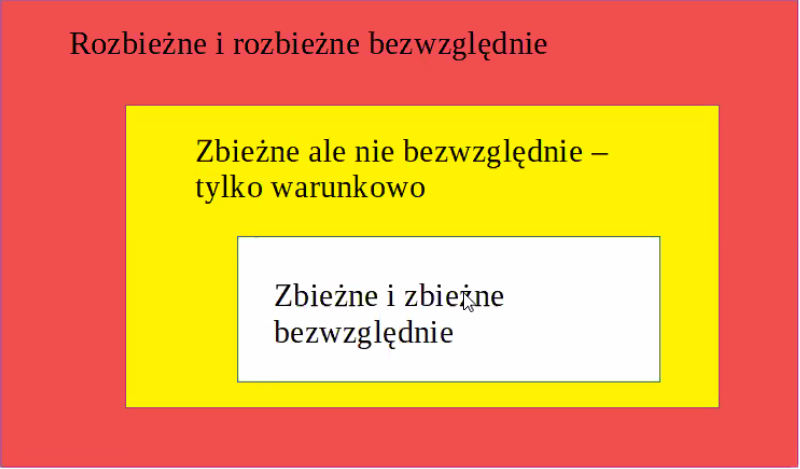
\includegraphics[scale=0.6]{img/rozbiezneirozbiezne.png} \\

\begin{przyklad}

Szereg $ \sum\limits_{n=1}^{\infty} \frac{\sin n}{\sqrt[3]{n^4}} $ jest zbieżny bezwzględnie, bo biorąc
$ \sum\limits_{n=1}^{\infty} \left| \frac{\sin n}{\sqrt[3]{n^4}} \right| $ i używając kryterium porównwawczego mamy

$$ 0 \leq \left| \frac{\sin n}{\sqrt[3]{n^4}} \right| = \frac{|\sin n|}{n^{\frac{4}{3}}} \leq \frac{1}{n^{\frac{4}{3}}} $$

a szereg $ \sum\limits_{n=1}^{\infty} \frac{1}{n^{\frac{4}{3}}} $ jest zbieżny, bo $ \frac{4}{3} > 1 $. 

Zatem
$ \sum\limits_{n=1}^{\infty} \left| \frac{\sin n}{\sqrt[3]{n^4}} \right| $, a stąd
$\sum\limits_{n=1}^{\infty} \frac{\sin n}{\sqrt[3]{n^4}}$ też jest zbieżny.
\end{przyklad}


\subsection*{Szeregi naprzemienne}
\addcontentsline{toc}{subsection}{Szeregi naprzemienne}

Są to szeregi, w których na zmianę dodajemy i odejmujemy wyrazy dodatnie:

$ a_{n_0} - a_{n_0 + 1} + a_{n_0 + 2} - a_{n_0 + 3} + ... $ \ lub \ $ -a_{n_0} + a_{n_0 + 1} - a_{n_0 + 2} + a_{n_0 + 3} + ...  $ \
gdzie $a_n > 0$. \\

Postać ogólna :

$ \sum\limits_{n = n_0}^{\infty} (-1)^n \cdot a_n $ \ lub \ $ \sum\limits_{n = n_0}^{\infty} (-1)^{n+1} \cdot a_n $ \\

\begin{przyklad}

$$ \sqrt{2} - \sqrt{3} + \sqrt{4} - \sqrt{5} + ... = \sum\limits_{n=2}^{\infty} (-1)^n \sqrt{n} $$

$$ 1 - \frac{1}{2} + \frac{1}{3} - \frac{1}{4} + ... = \sum\limits_{n=1}^{\infty} \frac{(-1)^{n+1}}{n} $$
\end{przyklad}

\begin{tw}{Twierdzenie}

Szereg naprzemienny $ \sum\limits_{n = n_0}^{\infty} (-1)^n \cdot a_n $ \ lub \ $ \sum\limits_{n = n_0}^{\infty} (-1)^{n+1} \cdot a_n $
nazywany jest \underline{szeregiem Leibnitza}, jeżeli $a_n$ jest ciągiem nierosnącym i zbieżnym do 0.
\end{tw}

Na przykład $ 1 - \frac{1}{2} + \frac{1}{3} - \frac{1}{4} + ... = \sum\limits_{n=1}^{\infty} \frac{(-1)^{n+1}}{n} $
jest szeregiem Leibnitza, bo tutaj $ a_n = \frac{1}{n} $ jest malejący i zbieżny do 0. \\

\subsection*{Twierdzenie (Leibnitz)}
\addcontentsline{toc}{subsection}{Twierdzenie (Leibnitz)}

Każdy szereg Leibnitza jest zbieżny. \\

Uwagi

\begin{itemize}
    \item Twierdzenie to daje tylko zbieżność warunkową, nie gwarantuje bezwględnej
    \item Gdy ciąg $a_n$ nie dąży do 0 to szereg naprzemienny $ \sum\limits_{n = n_0}^{\infty} (-1)^n \cdot a_n $ jest
    rozbieżny, gdyż $(-1)^n a_n$ też nie dąży do 0. Wynika to z twierdzenia

    $$ \lim_{n \to \infty} a_n = 0 \Leftrightarrow \lim_{n \to \infty} (-1)^n a_n = 0 \Leftrightarrow \lim_{n \to \infty} |a_n| = 0$$

    \item Wystarczy, by ciąg $a_n$ był nierosnący dla $ \forall n \geq k \geq n_0$.
    \item Gdy ciąg $a_n$ zbiega do 0 ale nie jest nierosnący to \textbf{NIC NIE WIEMY} o zbieżności szeregu.
    \item Do badania czy $a_n$ jest nierosnący można próbować rozszerzyć $a_n$ do funkcji $f$ tak by $f(n) = a_n$.
    Potem --- pochodna itd.
    Gdy szereg naprzemienny jest zbieżny bezwzględnie to tw. Leibnitza nie jest potrzebne. \\
\end{itemize}

\textbf{Ważna uwaga}

Poza twierdzeniem Leibnitza wszystkie pozostałe kryteria (porównawcze, ilorazowe, Cauchy'ego, d'Alemberta, całkowe, warunek konieczny) dają
albo \underline{dwie zbieżności} (zwykłą oraz bezwzględną) albo \underline{dwie rozbieżności} (zwykłą oraz bezwzględną)..

Nie pozwolą natomiast uzyskać zbieżności warunkowej. Tylko twierdzenie Leibnitza pozwoli taką zbieżność wykryć.

W przypadku kryterium porównawczego, ilorazowego lub całkowego wynika to z faktu, że działamy na szeregach o wyrazach nieujemnych, a więc
$ \suminfty{n_0} a_n = \suminfty{n_0} |a_n| $ \ i zbieżność bezwzględna jest równoważna zwykłej zbieżności.

W przypadku warunku koniecznego możemy jedynie wywnioskować rozbieżność a to oznacza też rozbieżność bezwzględną.

W przypadku kryterium Cauchy'ego lub d'Alemberta wynika to z własności modułu i faktu, że w obu tych kryteriach dla szeregów
\ $ \suminfty{n_0} |a_n| $ \ oraz \ $ \suminfty{n_0} a_n $ \ liczymy granicę tego samego wyrażenia :
$ \sqrt[n]{||a_n||} = \sqrt[n]{|a_n|} $ \ i podobnie \ $ \left| \frac{|a_{n+1}|}{|a_n|} \right| = \left| \frac{a_{n+1}}{a_n} \right| $
\vspace{20pt}

Dla $ a_n = \frac{(-3)^n}{n^3} $ \ i szeregu \ $ \suminfty{1} \frac{(-3)^n}{n^3} $ \ zarówno kryterium Cauchy'ego jak i d'Alemberta daje granicę
\[ \lim_{n \to \infty} \left| \frac{a_{n+1}}{a_n} \right| = \lim_{n \to \infty} \sqrt[n]{|a_n|} = 3 > 1 \]

Zatem ten szereg jest rozbieżny bezwzględnie i rozbieżny w zwykłym sensie.

Oznacza to także, że \ $ \suminfty{1} |a_n| = \infty $ \ natomiast jeśli chodzi o sumę \ $ \suminfty{1} a_n $ \ to nie mamy pewności czy istnieje
(wtedy jest nieskończona) czy też nie istnieje.

W powyższym przykładzie \ $ \suminfty{1} \frac{(-3)^n}{n^3} $ \ nie istnieje. Wynika to z ciekawej własności szeregów naprzemiennych i własność
ta pokazuje różnicę między kryterium Cauchy'ego i d'Alemberta. 
\vspace{20pt}

\begin{tw}{Twierdzenie}

Jeśli mamy szereg naprzemienny \ $ \suminfty{n_0} (-1)^n a_n, \ a_n > 0 $ i kryterium d'Alemberta daje rozbieżność, tzn.
$ \lim_{n \to \infty} \frac{a_{n+1}}{a_n} > 1 $ \ to suma \ $ \suminfty{n_0} (-1)^n a_n $ \ nie istnieje.
\end{tw}

\bigskip

Dla kryterium Cauchy'ego powyższe twierdzenie nie musi zachodzić, są przykłady szeregów naprzemiennych dla których z kryterium Cauchy'ego otrzymujemy
rozbieżność, a mimo to suma szeregu jest równa $\infty$.
\vspace{20pt}

\begin{blad}{Popularny błąd -- użycie kryterium Cauchy'ego / d'Alemberta i badanie obu typów zbieżności osobno}

" ... z kryterium Cauchy'ego / d'Alemberta wynika więc, że \ $ \suminfty{1} \frac{(-3)^n}{n^3} $ \ jest rozbieżny bezwzględnie.

\textcolor{red}{Ale może być jeszcze zbieżny normalnie. }

\textcolor{red}{Badam zwykłą zbieżność z twierdzenia Leibnitza...}"
\bigskip

\textbf{STRATA CZASU I ENERGII}. Jak już pisaliśmy, dla tych kryteriów mając rozbieżność bezwzględną mamy też zwykłą rozbieżność.
\end{blad}

\begin{blad}{Popularny błąd -- niepewne/błędne wnioski co do sumy szeregu rozbieżnego} 

"... z kryterium Cauchy'ego / d'Alemberta wynika więc, że $ \suminfty{1} \frac{(-3)^n}{n^3} $ jest rozbieżny \textcolor{red}{do $\infty$}"

\textbf{Niepewny wniosek}. Jeżeli szereg zawiera nieskończenie wiele wyrazów dodatnich i nieskończenie wiele wyrazów ujemnych to kryteria te
\textbf{nie gwarantują} istnienia sumy szeregu.

A poza tym w zadaniach typu "zbadać zbieżność szeregu" mamy jedynie określić czy suma jest skończona czy nie.
\end{blad}

\begin{blad}{Popularny błąd -- opisowne "badanie" monotoniczności ciągu, bez obliczeń}

Na przykład dla ciągu $ a_n = \frac{n}{1000n + 1} $ :

"Ciąg $a_n$ jest \textcolor{red}{malejący}, bo mianownik \textcolor{red}{szybciej rośnie niż licznik}."

GAME OVER... \ Takie "rozwiązanie" jest jak \textbf{pisanie bajek} --- nie musi mieć \linebreak
\textbf{nic wspólnego z prawdą}.

Dla powyższego ciągu mianownik rzeczywiście szybciej rośnie niż licznik (i to 1000 razy!), a mimo to ciąg ten jest rosnący.
\end{blad}

\begin{przyklad}

$$ \sum\limits_{n=2}^{\infty} \frac{(-1)^n \cdot \ln n}{n} $$

Tutaj $ a_n = \frac{\ln n}{n} $. Rozszerzamy go do funkcji $ f(x) = \frac{\ln x}{x}, \ x \geq 2 $.

$$ f'(x) = \frac{1 - \ln x}{x^2} < 0 \Leftrightarrow x > e \approx 2,72 $$

Zatem $f$ jest malejąca dla $ x \in (e, \infty) $ czyli $a_n$ jest malejący dla $n \geq 3$.

Ponadto

$$ \lim_{x \to \infty} f(x) = \lim_{x \to \infty} \frac{\ln x}{x} = \left[ \frac{\infty}{\infty} \right][H]
= \lim_{x \to \infty} \frac{\frac{1}{x}}{1} = 0 $$

Zatem $ \lim_{n \to \infty} a_n = 0 $.

Mamy więc szereg naprzemienny, który z tw. Leibnitza jest zbieżny.

Nie jest jednak zbieżny bezwzględnie bo dla $ \sum\limits_{n=2}^{\infty} \left| \frac{(-1)^n \cdot \ln n}{n} \right|
= \sum\limits_{n=2}^{\infty} \frac{\ln n}{n} $ mamy z kryterium porównawczego $0 < \frac{0,5}{n} < \frac{\ln n}{n}$,
a szereg $ \sum\limits_{n=2}^{\infty} \frac{0,5}{n} $ jest rozbieżny.

Jest to więc szereg zbieżny warunkowo.
\end{przyklad}

Podsumowanie : które kryterium zbieżności kiedy?

\begin{itemize}
    \item P --- porównawcze
    \item I --- ilorazowe
    \item C - Cauchy'ego
    \item A - d'Alemberta
    \item $\int$ --- całkowe
    \item ZB --- zbieżność bezwględna
    \item L - twierdzenie Leibnitza \\
\end{itemize}

\begin{table}[!htbp]
    \centering
    \begin{adjustbox}{width=0.9\textwidth}
    \begin{tabular}{|c|c|}
    \hline
    Wyrażenia występujące w $a_n$ & Sugerowane kryterium dla $ \sum\limits_{n=n_0}^{\infty} a_n $ \\[15pt] \hline
    Tylko potęgi $n$ lub pierwiastki z potęg $n$ & P \ \colorbox{yellow}{I} \ ale \colorbox{red}{NIGDY C A} \\[10pt] \hline 
    \underline{Te same} najwyższe potęgi $a_n$ w \underline{liczniku i mianowniku} & P \ \colorbox{yellow}{I} \ ale \colorbox{red}{NIGDY C A} \\[10pt] \hline
    \underline{Różne} najwyższe potęgi $a_n$ w \underline{liczniku i mianowniku} & P \ I \ \colorbox{yellow}{C \ A} \\[10pt] \hline
    funkcja złożona $ f(b_n), \ b_n \to 0 $ & \colorbox{yellow}{I} \ P \\[10pt] \hline
    n! & \colorbox{yellow}{A} \ P \\[10pt] \hline
    $n$ - ta sama potęga: $(...)^n$ & C \\[10pt] \hline
    Ciągi bez granicy, np. $\sin n$ & P \ (+ inne, gdy trzeba) \\[10pt] \hline
    $\ln n$ & \colorbox{yellow}{P} \ $\int$ \\[10pt] \hline
    $(-1)^n$ i ogólne $a_n$, o różnych znakach & ZB \ (+ inne, gdy trzeba) \ L \\[10pt] \hline
    \end{tabular}
\end{adjustbox}
\end{table}

\pagebreak

Przykłady do samodzielnego policzenia : \\

\begin{adjustbox}{width=0.7\textwidth}
    \begin{tabular}{ccc}
        $ \suminfty{1} \frac{\sqrt{n^2 + 3}}{n^3 + 2} $ & $ \suminfty{1} \frac{n^3 + 5}{n!} $ & $ \suminfty{1} \frac{2^n + 3^n}{n^2 \cdot 3^n + 1} $ \\
        \\
        $ \suminfty{1} \frac{2^n + 7 \cdot 3^n}{5^n - 4^n} $ & $ \suminfty{1} \left( \frac{2n+3}{3n+2} \right)^n $ & $ \suminfty{1} \arctan \frac{1}{\sqrt{n}} $ \\
        \\
        $ \suminfty{1} \frac{3 + \cos (n^2)}{\sqrt[3]{n}} $ & $ \suminfty{1} \frac{(-1)^n \cdot n}{n^2 + 2} $ & $ \suminfty{1} \frac{\cos (n^2)}{2^n} $
        \\
    \end{tabular}    
\end{adjustbox}